\section{Creating a BT structure}
    There are several possible approaches to creating a BT structure. We will present several of these approaches and state the used one. In this section we used the insight from \cite{BT_creation}.\\
    The first approach is creating the complete BT by hand. Meaning that human must desing every node and its position and function within the structure.\\
    The second approach is crating an initial BT and let RL algorithms improve its functionality and optimality. There are a few options in this approach.\\
    The third possible approach is constructing the BT from a previously recorded human behavior.\\
    The last possible approach lets the RL algorithm construct the BT structure from scratch.\\\\
    \bfc{Chosen approach}\\
    We have chosen to use the first approach, meaning we will construct the whole tree structure by hand. This was done as it is the easiest approach to this task, and it does not require any additional steps.\\
    Using different approaches to designing and improving the BT structru may be an interesting task for future work.\\
    We will design the BT structure in the GUI application, designed alongside our chosen BT library, Groot. The application interface is shown in figure \ref{fig:groot}.
    \begin{figure}[ht]
        \centering
        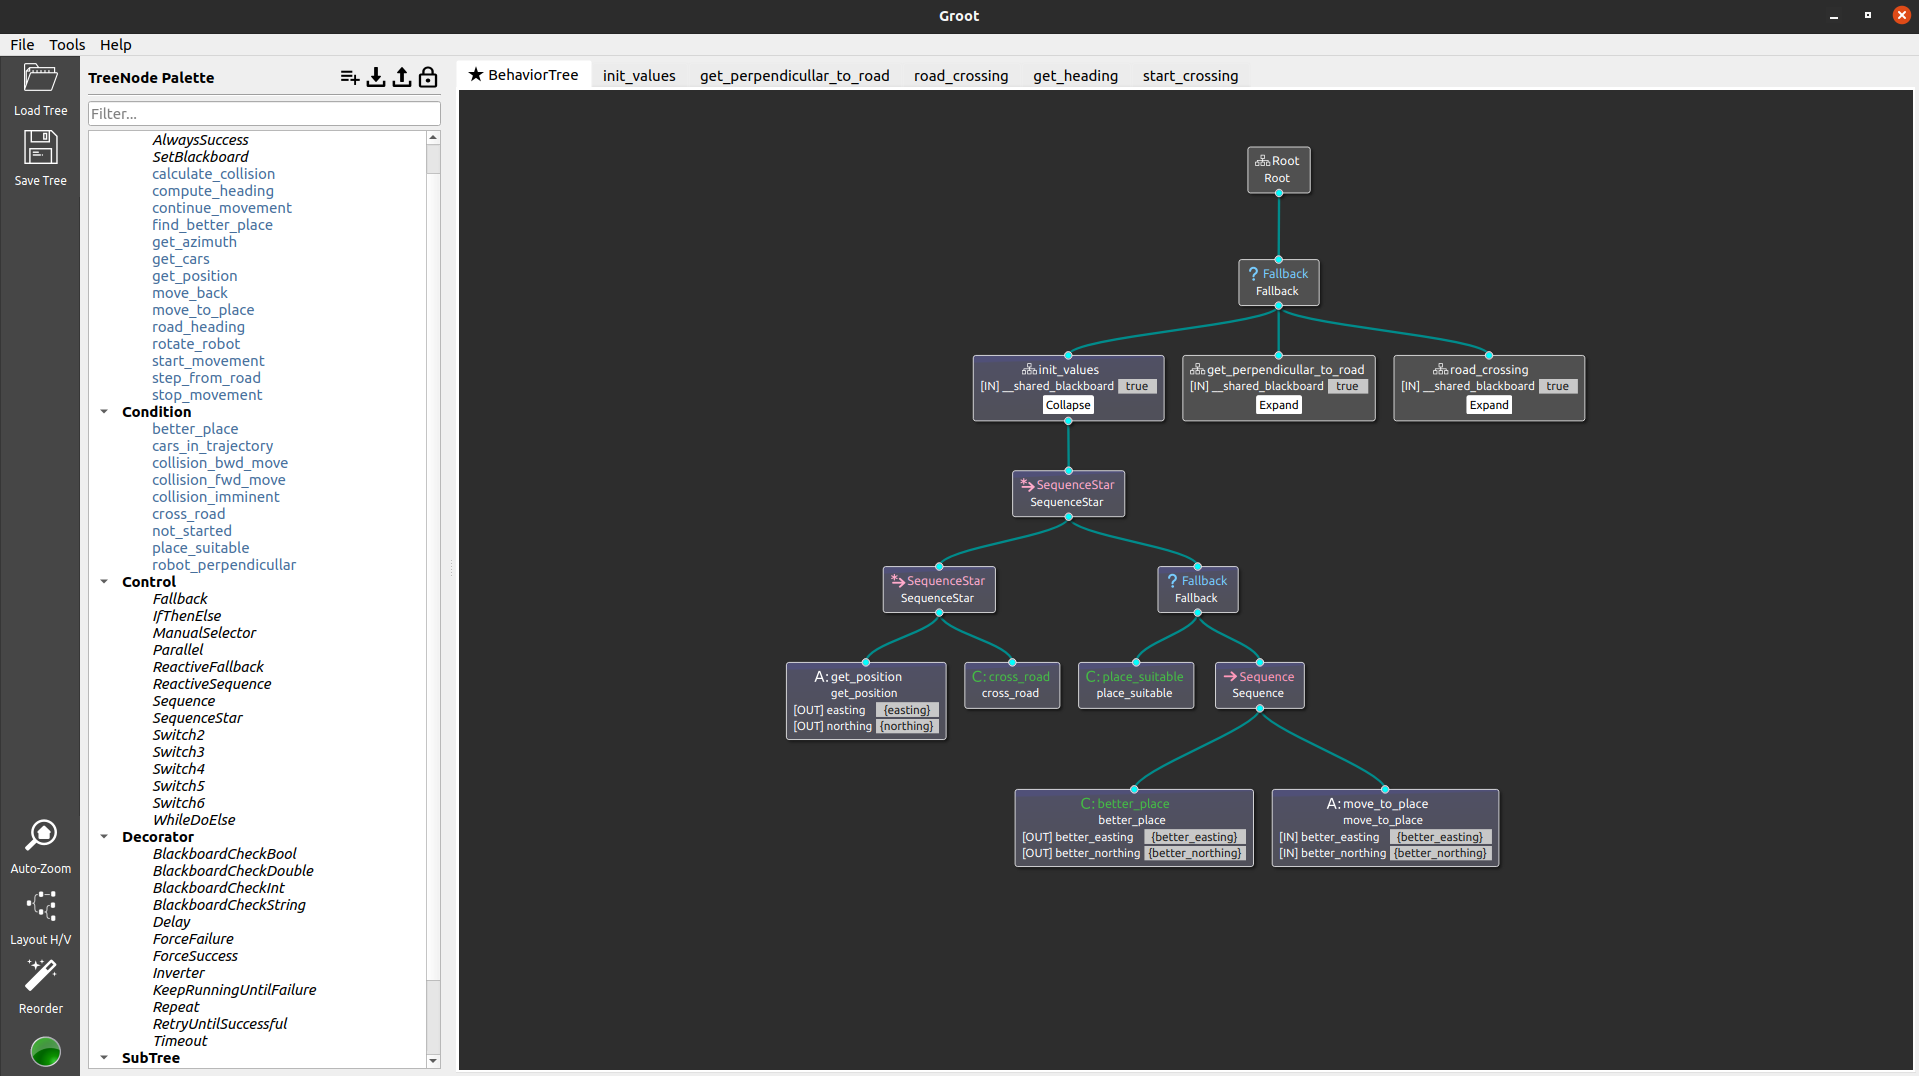
\includegraphics[width=\linewidth]{images/Groot.png}
        \caption{The Groot application interface.}
        \label{fig:groot}
    \end{figure}

\section{Structure hierarchy}
    We will devide the whole tree structure into several sub-trees to help with readibility, modularity and maintainability.\\
    The first sub-tree will help with intitialization and will be responsible for determining whether the tree should be run or not. It is also responsible for navigating the robot into a suitable place for crossing. This sub-tree will be called \texttt{Init-BT}.\\
    The second sub-tree will be responsible for positioning the robot such that it is perpendicullar to the road it is trying to cross. This sub-tree will be called \texttt{Perpendicullar-BT}.\\
    The third sub-tree will be responsible for the navigation of thr robot during the crossing. It will check the positions and speed of incomming traffic, and determine the best strategy for the crossing. This sub-tree will be called \texttt{Crossing-BT}.\\
    There are a few more sub-trees in our structure, but those are not that important to write about here. They will be presented, when they are mention in the main sub-trees structure. The main task that they serve is to help with modularity and reusability of the behavior they encode.
    The main BT is shown in figure \ref{fig:main-BT}.
    \begin{figure}[ht]
        \begin{tikzpicture}[sibling distance=30mm, minimum width=1cm, minimum height=0.8cm]
            \node [draw] {$Root$}
                child {node [draw] {$\to$} edge from parent [-{Stealth[length=2.5mm]}]
                child {node [diamond, draw, aspect=2.3, xshift=0-1cm, yshift=0-0.5cm] {Init-BT}}
                child {node [diamond, draw, aspect=2.9, yshift=0-0.5cm] {Perpendicullar-BT}}
                child {node [diamond, draw, aspect=2.3, xshift=1.5cm, yshift=0-0.5cm] {Crossing-BT}}};
        \end{tikzpicture}
        \caption{Main BT structure.}
        \label{fig:main-BT}
    \end{figure}

\section{Init-BT}
    As mentioned earlier this BT is responsible for determining if we should start the crossing or not, and navigating the robot to optimal location for doing so. This tree will be executed only once for each crossing, we acomplish this with a \texttt{SequenceStar} node as the first node after \texttt{Root}. The \texttt{Init-BT} structure is shown in figure \ref{fig:Init-BT}.
    \begin{figure}[H]
            \begin{tikzpicture}[sibling distance=28mm, minimum width=1cm, minimum height=0.8cm]
                \node [draw] {$Root$}
                    child {node [draw] {$\to^{*}$} edge from parent [-{Stealth[length=2.5mm]}]
                    child {node [ellipse, draw, xshift=0-0.4cm] {StartAlgorithm}}
                    child {node [draw] {$\to^{*}$}
                    child {node [draw, xshift=0-2.5cm] {GetPosition}}
                    child {node [ellipse, draw, xshift=0-2.5cm] {CrossRoad}}}
                    child {node [draw] {?}
                    child {node [ellipse, draw, xshift=1.1cm] {PlaceSuitable}}
                    child {node [draw, xshift=1cm] {$\to$}
                    child {node [ellipse, draw, xshift=0-1.1cm] {BetterPlace}}
                    child {node [draw, xshift=0-0.6cm] {MoveToPlace}}}}};
            \end{tikzpicture}
            \caption{The Init-BT structure.}
            \label{fig:Init-BT}
        \end{figure}
